\documentclass[10pt]{scrartcl}
%\documentclass[11pt]{scrartcl}

\usepackage{url,pdfpages,moreverb,color}
\definecolor{cscolour}{rgb}{0.5,0.1,0.1}

\title{Notes for exam question authors}
\author{Norman Gray}
\date{Version exam-n-1.4.0, 2022 October 10}

\parindent=0pt
\parskip=\medskipamount

\makeatletter
\def\cs@arg#1{\texttt\{\textit{#1}\texttt\}%
  \advance\@tempcnta-1
  \ifnum\@tempcnta>0
    \let\next\cs@arg
  \else
    \let\next\endgroup          % begun in \cs
  \fi
  \next}
{\catcode`\|=0 \catcode`\\=12
|gdef|cs@textbackslash#1{|texttt{\#1}}}
% \cs{foo} typeset \foo
% \cs[2]{foo}{bar}{baz} typeset \foo{bar}{baz}
\newcommand\cs[2][0]{\begingroup
  \color{cscolour}%
  \cs@textbackslash{#2}%
  \@tempcnta=#1
  \ifnum\@tempcnta>0
    \let\next\cs@arg
  \else
    \let\next\endgroup
  \fi
  \next}

\let\origvec\vec
% We'd like to say here
%   \newif\ifexamn@uprightpi \examn@uprightpitrue
% but that's not supported for CM fonts
\usepackage{examndefs}

\makeatother

\def\env#1{\texttt{\textcolor{cscolour}{\{#1\}}}}
\def\opt#1{\texttt{[#1]}}
\def\package#1{\textsf{#1}}

\setcounter{secnumdepth}0

\begin{document}
\maketitle

The full documentation for the \texttt{exam-n} document class is in
the file \texttt{exam-n.pdf}, but some of this is quite detailed, and
addressed to the exams convener, who has to assemble the overall
exam.  This document is a compact account of how to use the exams
class as a question author.

You can find updated versions of the \texttt{exam-n} document class, and the
complete documentation, at \url{http://purl.org/nxg/dist/exam-n}.

\subsection{Template}
\label{s:template}
\listinginput1{template-question.tex}

Notice first that this is a standalone document -- you can \LaTeX\ it
to produce a formatted exam paper, as long as you include the
\opt{compose} option in the document class line.  This complete
document can later be given to the exams convener, who can
input it unchanged into the master file which pulls the various questions
together.  It follows from that that you should be hesitant about putting anything into
the preamble other than \cs{usepackage} commands, and you should
consult with the exams convener to ensure that such packages go into
the master file, too.  It's probably a safe bet that the `graphicx'
package will be included in the master file.  If you want to include
a \cs{newcommand}, or anything like that,
it can be placed inside the \env{question} environment.  For
other customisations, negotiate with the exams convener.

The \env{question} environment contains (surprise) a question, broken into
parts (a, b, c, \dots) by \cs{part} commands, and with the distribution of marks within
the question being indicated by \cs[1]{partmarks}n; the class will check that the
marks in \cs{partmarks} do add up to the question goal given as an
argument in \cs[1]{begin\{question\}}{markgoal}.  Within the
question there can be one or more \env{solution} environments, which are
not displayed in the final version (obviously), but which do appear in
draft modes.  You'll most typically have a \cs{partmarks} macro and a
\env{solution} environment for each \cs{part}, but they don't have to
match up, and you can have the entire solution at the end if you prefer.

The \cs{partmarks} command will most typically go at the end of a
paragraph, but it may also appear inside an equation (that is, in
\verb|\[...\]|; don't use \verb|$$...$$|), inside one or other
\package{amsmath} display environments, or in a list or other
environment.  If it appears inside an environment, the indicator will
appear at the \emph{end} of the environment, independent of where in
the environment the command was typed (which implies that you can't
have more than one inside an environment).

The starred version is similar, but budges its indicator upwards
a little, and is a heuristic alternative which is useful in some
cases \emph{after} a list or display, or after a numbered equation, if the placement of the
indicator is otherwise inaesthetic
(if the style of the part-marks indicators happens to be such
that the indicator may be mistaken for an equation number, then
it would be wise to use either \cs{partmarks} or \cs{partmarks*}
after the equation, instead).  If you use \cs{partmarks*} within a
display, you might be confronted by an error message, talking
about \cs{eqno} in maths mode, which is even more incomprehensible
than most \LaTeX\ messages.

Note that \cs{partmarks} ends a paragraph (\cs{partmarks*} doesn't): this is
probably good style, but if you insist on mid-paragraph marks, then a following
\verb|\noindent| will be useful.  It's helpful to use \cs{partmarks} inside a
\env{solution} to indicate the distribution of marks -- this doesn't mess up
the mark-totalling calculation.

You may optionally give a question number as an argument to the
\env{question} environment: \cs[1]{begin\{question\}[n]}{markgoal}.
In \opt{compose} mode, this simply sets the question number, but in the other
modes, when the question file is included in a master file, this
checks that the given number~$n$ is what would be assigned
automatically, to help detect missing or out-of-order questions.  If
the question identifier is not a number, such as `D1', then you can
provide that identifier here also, but in this case you must also set
\cs{QuestionNumberChecksOff} in the question preamble.

The \cs{partmarks} command has an optional argument which
indicates the category of the question, thus `bookwork', `unseen',
and so on.  If this is present -- for example
\cs[1]{partmarks[bookwork]}{5} -- then the category is included in the
marks indicator.
As you might hope, the \cs{partmarks*} command can take this
optional argument also: \cs[1]{partmarks*[bookwork]}{5}.
This extra text will typically be only one or two words long, but if
the text is much longer than that, it will be turned into a footnote.

One common exam or test question type is a multiple-choice question.
This is indicated by a \cs{begin\{mcq\}} environment, which contains a
textual question followed by a sequence of possible answers indicated by
\cs{item}, including precisely one correct answer, indicated by
\cs{answer} (this is of course formatted identically to the others,
unless the \opt{showsolutions} option is present).  Before you can use
the \env{mcq} environment, you must call
\cs[1]{multiplechoiceanswers}{n} to indicate how many options are
required in each question.
It's OK to have a \env{solution} within an \env{mcq} environment,
perhaps to provide commentary on or explanation of the correct answer.

You can include a \env{questiondata} environment at (typically) the end of
the question: this is intended for extra equations or constants which
are useful for the examinee.

The \env{figure} and \env{table} environments act differently from the
way they usually act in \LaTeX: \emph{`floats' don't float}.  In each
case, the content is forced to be always `here', and in addition is
also tied to the text which follows it, so that a page break will not
occur immediately after a figure or table.  There are \emph{no} figure
or float options permitted in this class's `floating' environments
(that is, option \texttt{[h]} is neither necessary nor permissible).
If you need to tune the page breaking, then you should use
\verb|\goodbreak|, \verb|\vspace| or, in extremis, \verb|\newpage|.
The \cs[1]{caption}{text} command works as usual; the figure and table
numbering sequences continue through the solutions, if they're shown,
but this isn't expected to be a problem.

There is neither a \env{figure*} nor a \env{table*} environment,
because this is a single-column class.
Use the no-option unstarred versions instead.

\subsection{Hints}

Figures can be included with \cs{includegraphics} as usual, as long as
the \package{graphicx} package has been included at the top of the master
file.  If you want to include complete pages from a PDF (most
typically containing a scanned handwritten model answer), then you can
do so by including the \package{pdfpages} package at the top of the file, and
then \cs[1]{includepdf[pages=\{-\}]}{filename} inside a \env{solution}
environment.
The \texttt{pages=\{-\}} option means that all pages from the file are
inserted; you may wish to use \texttt{scale=0.8} to shrink the PDF;
the option \verb|pagecommand={\thispagestyle{fancy}}| will cause the other
class apparatus, such as page numbers and headers, to be
superimposed on the included pages.
See the documentation of the \package{pdfpages} package for more information.

If you use \cs{label} within a \env{question} environment, that label
will, as you might expect, refer to the question number.

Include marginal notes with \cs[1]{comment}{remark} -- these show up in drafting
modes (\opt{draft} and \opt{compose}), but not in the final version.
The \cs[1]{author}{name} command is just
a type of comment.  If you need to make more noise, then
\cs[1]{shout}{remark} inserts a highlighted \emph{remark} in the flow of text
(so it can be used anywhere) and includes the remark in a prominent
list of exclamations at the end of the document.  Note that \cs{shout}
text \emph{appears in the \opt{final} version}: it is to draw
attention to problems (for example \cs[1]{shout}{solution wrong!})
which must be resolved before the exam is presented to students.

At the bottom of each page, you see a faint identification code, such
as `QM/123-456'.  This consists of an exam identifier, extracted from
the exam preamble, plus a code which changes each time \LaTeX\ is
run, but which is otherwise meaningless.
This helps you avoid collation accidents, and to distinguish
between slightly different versions of the printed document.

\subsection{Various convenience commands}
\label{s:othercommands}

Macro \cs[1]{vec}{v} is redefined to give bold-font vectors
rather than vectors with arrows, which is the (weird) \LaTeX\ default
-- thus $\vec v$ rather than $\origvec v$.
This is intended to work for bold greek as well as roman,
but it does so reliably only for the \opt{mtpro2} and \opt{stix2}
options.

Macros \cs{dd} and \cs{ddd}: \cs{dd} is a roman d, as used for
differentials; \cs{ddd} is the same with a preceding thinspace,
as used within integrals; for example
\[
 \verb|\int f(x)\ddd x = \int f(x)\,\dd x| = \int f(x)\ddd x
\]

You can typeset derivatives neatly:
\begin{center}
\def\dd{\mathrm{d}}
\begin{tabular}{rl}
\verb|\Diffl{a}{b}|     & $\displaystyle \Diffl ab$ \\[3ex]
\verb|\Diffl[2]{a}{b}|  & $\displaystyle \Diffl[2]ab$\\[3ex]
\verb|\Diffl*{a}{b}|    & $\Diffl* ab$ \\[2ex]
\verb|\Diffl*[2]{a}{b}| & $\Diffl*[2]ab$\\
\end{tabular}
\end{center}
The unstarred versions are for displayed equations, the starred
ones for inline maths.
There is analogous support for partial derivatives with \cs[2]{Partial}ab.

You should generally type units, and numbers with units, using the
\package{siunitx} package (use the \opt{siunitx} \cs{documentclass} option).

However this package currently also
supports a basic \verb|\units| command, described here.  This macro
is very likely to be removed in a future version of this package.
Macros \cs[1]{units}{expr}, \cs[1]{units*}{expr}: These typeset
physical units in an upright shape, with tilde or dot acting as a
separator between units.  Since this is typeset in maths mode, all
other spacing is ignored.  For example, \verb|$v=10\units{m.\mu s^{-1}}$|
gives $v=10\units{m.\mu s^{-1}}$.  The unstarred version includes some
leading space; the starred version can be used when referring to the
unit by itself, where it is not qualifying a number (eg labelling an
axis with units \verb|$B/\units*T$|, or $B/\units*T$).

The command \cs{e} sets an upright~`e':
\verb|$\e^{i\pi} + 1 = 0$| produces $\e^{i\pi} + 1 = 0$.
Other shortcuts may be available in customisations of this class.\footnote{%
The package used to support an \cs{au} macro, for astronomical
unit, and \cs{lambdabar} for Compton wavelength, but these have
since been removed.  The former is available via \package{siunitx}.}

Note: $\pi$ is set as an italic pi character, matching the
\LaTeX\ default.  Since it's (usually) used as the circular constant,
it should more properly be set upright, and you can get that using the
\opt{uprightpi} option.  This option also defines a \verb|\italicpi|
command, for completeness.  This option is at present
implemented only for the \opt{mtpro2} and \opt{stix2} options.

\subsection{Extra: Creating complete exams}
\label{s:complete}
As a question author, you are typically only concerned with one or two
single questions, and that is why this brief guide concentrates
exclusively on the \opt{compose} mode.  But you might be interested to see
how your text appears in the final exam.  A template master file is
below.  For more detail, see the complete documentation in \texttt{exam-n.pdf}.
\goodbreak
\listinginput1{template-master.tex}

The \texttt{exam-n} class currently supports a sample class option \opt{myclass}.
This automatically includes a suitable constants sheet in the
formatted paper.

On the following pages, you can see the result of \LaTeX ing the sample file on
p.\pageref{s:template}, and of processing the master file above.
As you can see, the \opt{compose} mode by default shows solutions,
and collects the \cs[1]{shout}{text} remarks to the end.
In the \opt{final} mode (which is the default mode), solutions
disappear, but the shouted-out alerts remain, just to make sure no-one
can miss them.
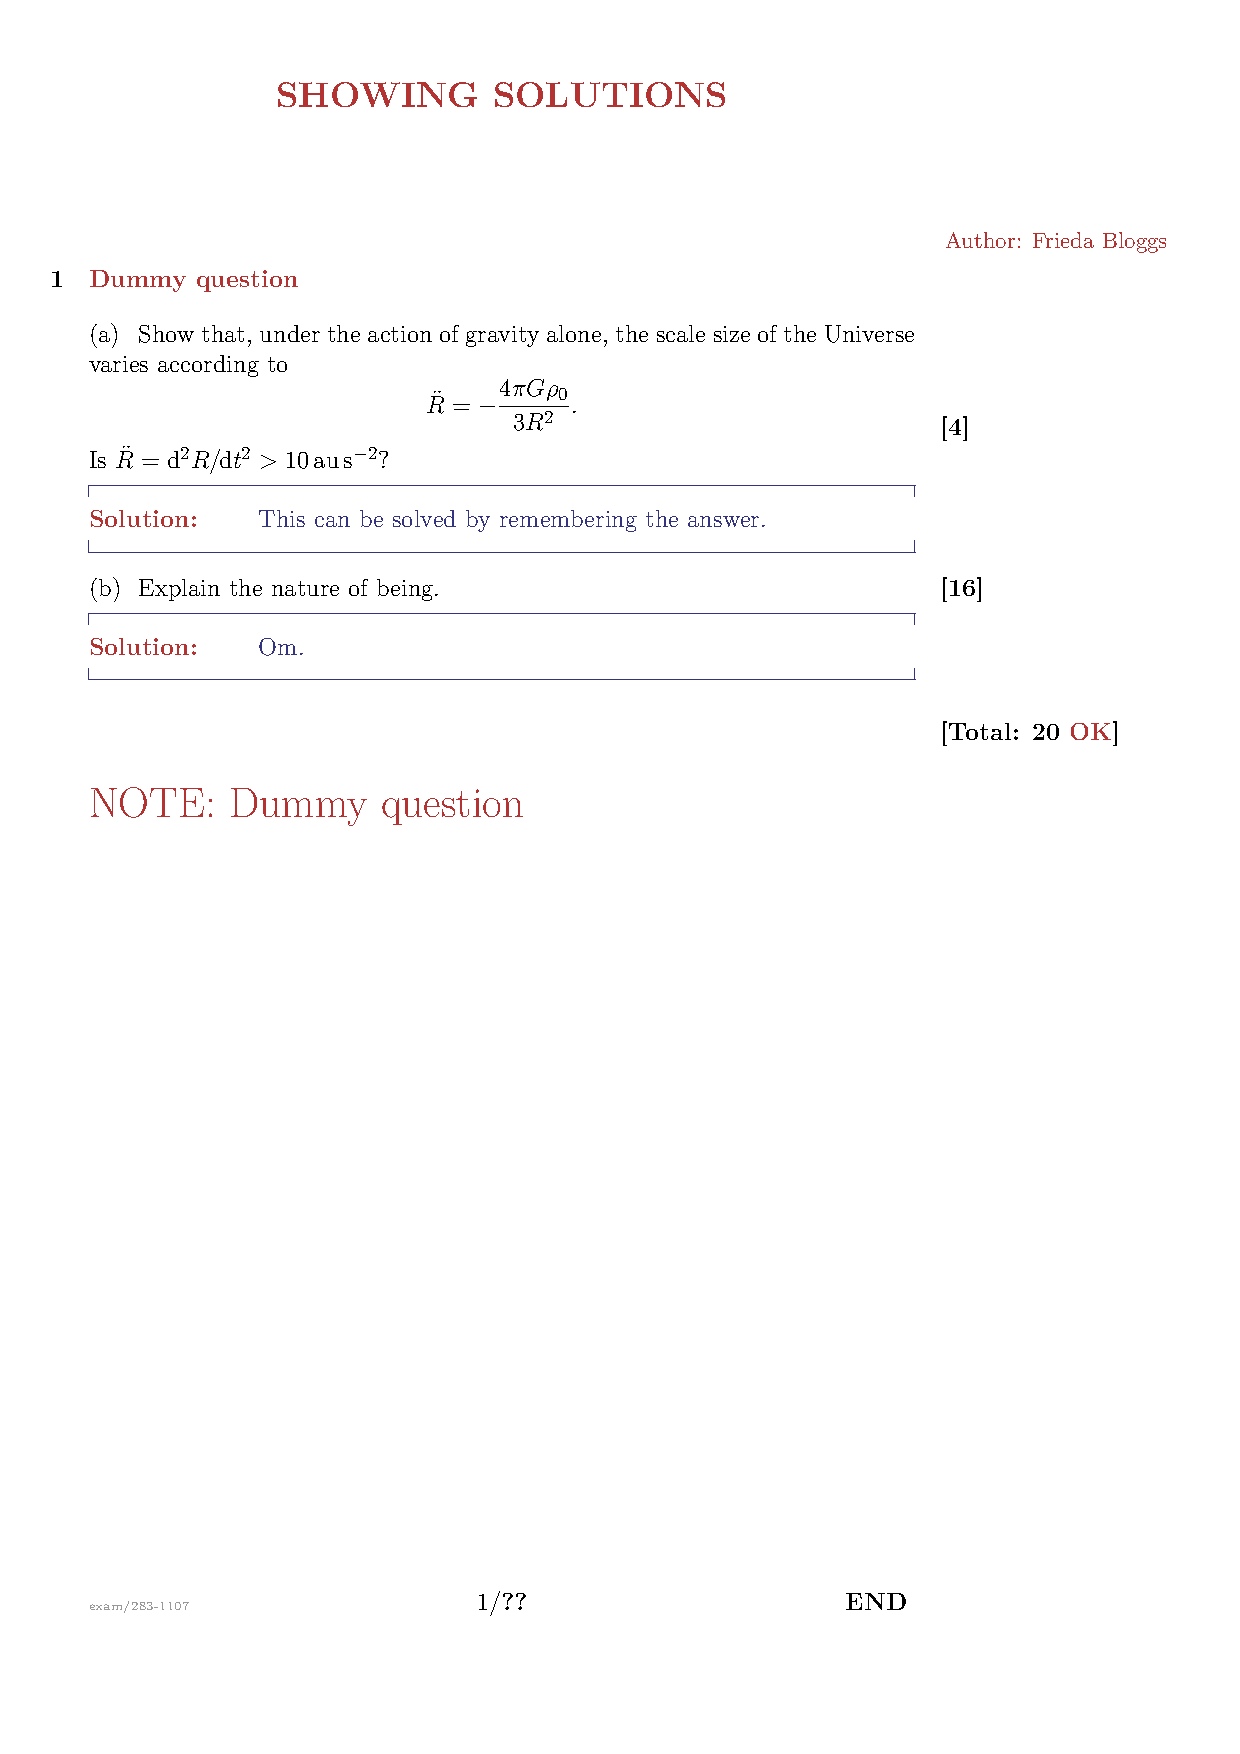
\includepdf{template-question.pdf}
\includepdf[pages={2,1},angle=90,nup=1x2,column]{template-master.pdf}
\end{document}
